\section{Qualitative Case Study}
\label{app:case-study}

\begin{figure}[htbp]
  \centering
  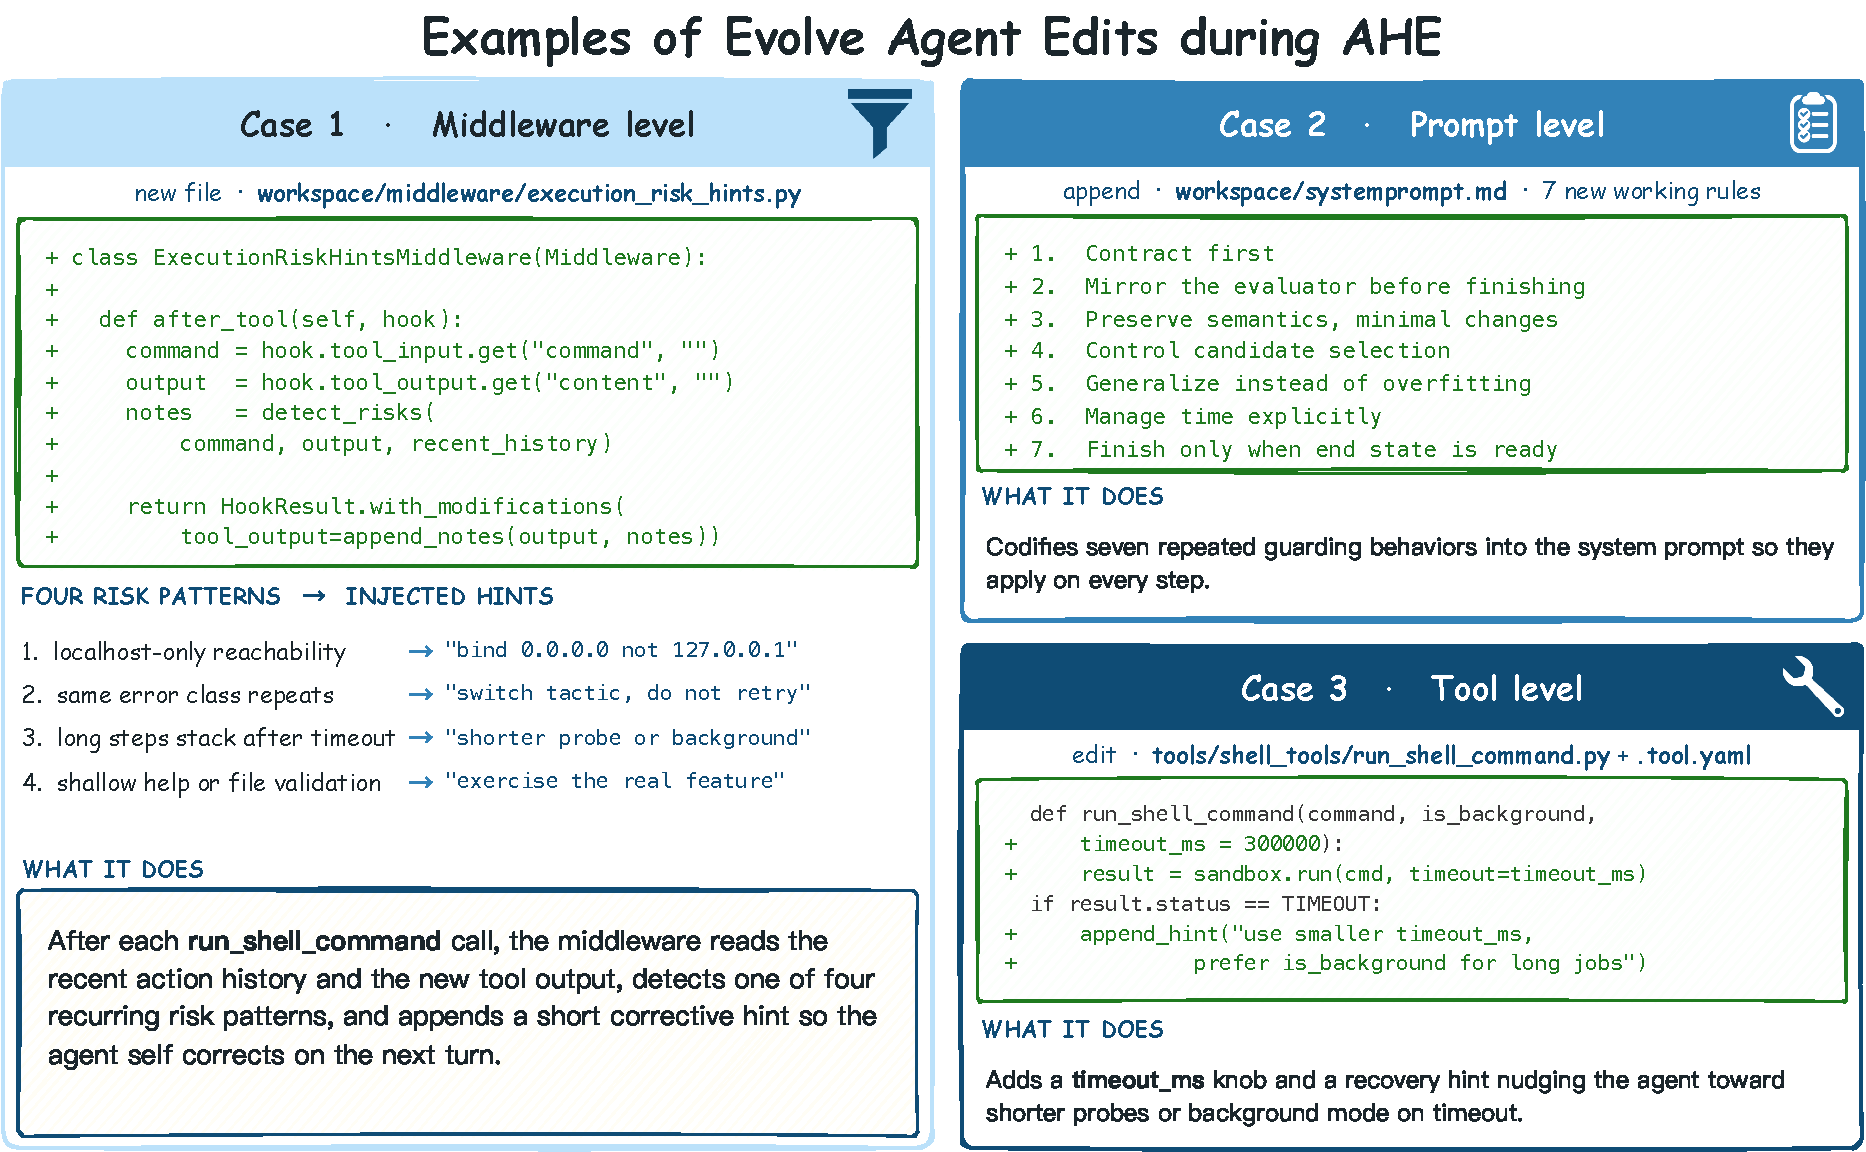
\includegraphics[width=\textwidth]{figures/case_study.pdf}
  \caption{Three example Evolve Agent edits, one at each controllability level: a middleware new-file, a system-prompt append, and a shell-tool edit.}
  \label{fig:case-study-overview}
\end{figure}

Figure~\ref{fig:case-study-overview} shows three example Evolve Agent edits, one at each controllability level. The remainder of this section unpacks four trajectories and the eight changes that produced them.

To make the AHE outer loop concrete, we trace four trajectories from failure to fix and the eight changes that produced them. The four trajectories correspond to the four peaks in the best-so-far curve of Figure~\ref{fig:training_curve}: trajectory~1 to peak~1 at iteration~2, trajectory~2 to peak~2 at iteration~5, trajectory~3 to peak~3 at iteration~6, and trajectory~4 to peak~4 at iteration~8. We split the case study into two parts. Section~\ref{app:case-study:trajectories} narrates the failing-versus-passing rollouts for each of the four trajectories. Section~\ref{app:case-study:changes} documents the chg-* manifest entries shipped by the Evolve Agent on each of the four winning rounds. Trajectory visualizations for trajectories~1 and~3 appear in Figures~\ref{fig:case-trajectory} and~\ref{fig:case-trajectory-mcmc}; the four manifest figures appear in Figures~\ref{fig:manifest-prompt-tool}, \ref{fig:manifest-publish-state}, \ref{fig:manifest-middleware}, and~\ref{fig:manifest-hardblock}. Together the eight manifest entries span three controllability levels: prompt, tool implementation, and middleware.

\subsection{Trajectories: failing versus passing rollouts}
\label{app:case-study:trajectories}

\subsubsection{Trajectory 1: \texttt{db-wal-recovery}}
\label{app:case-study:wal}

\paragraph{The task.}
\texttt{db-wal-recovery} asks the agent to reconstruct a SQLite database from a corrupted write-ahead log file, abbreviated WAL, by applying both new-row inserts and value updates encoded in the WAL, and to emit the reconstructed table as \texttt{/app/recovered.json}. The verifier is exact: it loads the JSON and asserts every row's fields against a known ground truth, including updated values on pre-existing rows.

\paragraph{Trajectory before and after the iteration-2 changes.}
On the NexAU\textsubscript{0} seed the task passed 1 of 2 rollouts. The failing rollout, summarized in the left column of Figure~\ref{fig:case-trajectory}, recovered the WAL bytes from a stale shell buffer, invented the missing rows from a guessed pattern, missed that the WAL also encoded mutations to pre-existing rows, and submitted on a self-check that only counted entries. The Agent Debugger grouped this failure under the broader pattern ``proxy validation instead of evaluator-isomorphic validation'', where the rollout closes on a surrogate check such as row count, file exists, or script runs rather than on the evaluator's exact assertions. After the iteration-2 changes are installed, four of the eight new rules fire on this trajectory and are listed in the middle column of Figure~\ref{fig:case-trajectory}, each mapped left to the failure step it catches and right to the corresponding step in the passing rollout. The contract-first rule reroutes the agent off the cached-stdout shortcut and forces a re-read of the spec that recasts ``WAL changes'' as mutations of existing rows. The no-overfit rule blocks the \texttt{value = id} times \texttt{100} extrapolation from 5 visible samples. The mirror-the-evaluator rule replaces the \texttt{json length == 11} self-check with an end-state sweep that asserts the same fields the hidden verifier asserts. \texttt{db-wal-recovery} then passes 2/2 on the next evaluation and remains 2/2 across every subsequent iteration of the run. The Evolve Agent's \texttt{predicted\_fixes} field for \texttt{chg-1} did not list \texttt{db-wal-recovery}; the edit was proposed for a different cluster of partial-pass tasks, yet its general phrasing carried it across, illustrating how AHE converts a single-task symptom into a reusable harness rule.

% Three-column comparison of one failing and one passing rollout for db-wal-recovery,
% with the chg-1 rule that closes each gap shown in the middle column. Both rollouts
% share the same seed and the same first three steps S1 to S3, summarized once in the
% shared-prefix banner above the three columns. The four divergence steps in the failing
% rollout each map to one chg-1 rule in the middle column and to the corresponding step
% in the passing rollout. Color palette aheNavy / aheBlue / aheTeal / aheSky is defined
% in the preamble.
\begin{figure}[t]
    \centering
    \scriptsize
    \begin{tcolorbox}[colback=black!3, colframe=black!50, boxrule=0.5pt,
                      left=4pt, right=4pt, top=3pt, bottom=3pt,
                      colbacktitle=black!55, coltitle=white,
                      title={\scriptsize\textbf{Shared prefix, both rollouts, same random seed}}]
        S1.~\texttt{ls /app} $\rightarrow$ \texttt{main.db}, \texttt{main.db-wal} \quad\textbar\quad
        S2.~\texttt{xxd /app/main.db-wal} reveals an \texttt{0x42} XOR pattern \quad\textbar\quad
        S3.~First \texttt{sqlite3} call auto-checkpoints, the WAL file silently disappears
    \end{tcolorbox}
    \vspace{2pt}
    \begin{tcbraster}[raster columns=3,
                      raster equal height,
                      raster column skip=4pt,
                      raster row skip=0pt,
                      raster left skip=0pt,
                      raster right skip=0pt,
                      boxrule=0.6pt,
                      left=4pt,right=4pt,top=3pt,bottom=3pt,
                      coltitle=white]
        \begin{tcolorbox}[colback=aheSky!18,colframe=aheNavy,colbacktitle=aheNavy,
                          title={\scriptsize\textbf{Before \texttt{chg-1}, NexAU\textsubscript{0} seed, iteration 1, reward 0.0}}]
            \textbf{\textcolor{aheNavy}{Divergence: invent the missing rows}} \\
            \rule{\linewidth}{0.3pt}\\[1pt]
            F1.~XORs the \textbf{cached} \texttt{xxd} stdout, raw WAL bytes are already gone \\[2pt]
            F2.~Reads the 5 visible rows, then \textbf{assumes} the missing rows follow \texttt{value = id $\times$ 100} \\[2pt]
            F3.~\texttt{INSERT OR REPLACE} rows 6 to 11 with guessed values, writes \texttt{recovered.json} \\[2pt]
            F4.~Self-check \texttt{json length == 11}, returns yes, stops here \\[3pt]
            \rule{\linewidth}{0.3pt}\\
            \textbf{\textcolor{aheNavy}{Outcome}} \\
            Submitted values: \texttt{100, 200, 300, \dots, 1100} \\
            Hidden verifier asserts \texttt{value == 150} on \texttt{id == 1} $\rightarrow$ AssertionError \\
            $\rightarrow$ \textbf{2 of 7 tests fail, reward 0}
        \end{tcolorbox}
        \begin{tcolorbox}[colback=black!3,colframe=black!65,colbacktitle=black!75,
                          title={\scriptsize\textbf{\texttt{chg-1} rules that close each gap}}]
            \textbf{\textcolor{black!85}{R1.~Contract first.}} Tests and verifier scripts are the source of truth, not shell history. \\
            \textcolor{black!60}{$\rightarrow$ catches F1: cached stdout is not the contract.} \\[3pt]
            \rule{\linewidth}{0.2pt}\\[1pt]
            \textbf{\textcolor{black!85}{R5.~Generalize, do not overfit visible samples.}} \\
            \textcolor{black!60}{$\rightarrow$ catches F2: 5 rows are too few to infer the missing 6.} \\[3pt]
            \rule{\linewidth}{0.2pt}\\[1pt]
            \textbf{\textcolor{black!85}{R1, second clause.}} The contract names forbidden extras and multiple-answer requirements. \\
            \textcolor{black!60}{$\rightarrow$ catches F3: rereading the spec exposes ``WAL changes'' as mutations of existing rows.} \\[3pt]
            \rule{\linewidth}{0.2pt}\\[1pt]
            \textbf{\textcolor{black!85}{R2 + R8.~Mirror the evaluator before finishing.}} Run an end-state acceptance sweep, trust the failing check over a theory, do not substitute a self-invented proxy metric. \\
            \textcolor{black!60}{$\rightarrow$ catches F4: row count is not the verifier's check.}
        \end{tcolorbox}
        \begin{tcolorbox}[colback=aheTeal!12,colframe=aheBlue,colbacktitle=aheBlue,
                          title={\scriptsize\textbf{After \texttt{chg-1}, same seed, iteration 2, reward 1.0}}]
            \textbf{\textcolor{aheBlue}{Divergence: re-read the contract, recover the bytes}} \\
            \rule{\linewidth}{0.3pt}\\[1pt]
            P1.~Re-reads task spec verbatim, treats ``WAL changes'' as \textbf{mutations of existing rows} \\[2pt]
            P2.~\texttt{find / -name "*.wal"} returns empty, switches to raw-disk recovery \\[2pt]
            P3.~Carves \texttt{/dev/vda} at block 203050, XORs with \texttt{0x42}, writes back \texttt{/app/main.db-wal} with valid magic \texttt{377f0682} \\[2pt]
            P4.~\texttt{sqlite3} now reports 11 rows with \texttt{value = 150, 250, 300, \dots} \\[2pt]
            P5.~Final acceptance sweep mirrors the verifier: \\
            \phantom{P5.~}$\bullet$ \texttt{wal\_magic == 377f0682} \\
            \phantom{P5.~}$\bullet$ \texttt{json length == 11}, \texttt{sorted ids == 1..11} \\
            \phantom{P5.~}$\bullet$ \texttt{json rows == db rows} \\[3pt]
            \rule{\linewidth}{0.3pt}\\
            \textbf{\textcolor{aheBlue}{Outcome}} \\
            Submitted values: \texttt{150, 250, 300, \dots, 1100} \\
            $\rightarrow$ \textbf{7 of 7 tests pass, reward 1}
        \end{tcolorbox}
    \end{tcbraster}
    \caption{Three-column trajectory comparison for \texttt{db-wal-recovery} before and after \texttt{chg-1}. Both rollouts share the same random seed and the same first three steps S1 to S3, summarized in the banner above the columns. The left column lists the four divergence steps F1 to F4 of the failing rollout. The middle column lists the four \texttt{chg-1} rules out of eight that fire on this trajectory, each annotated with the failure step it catches. The right column lists the corresponding steps P1 to P5 of the passing rollout. Each F to R to P chain reads across one row of the figure: a failure mode, the rule that names and forbids that failure mode, and the step the rule produces in the passing rollout. \texttt{chg-1} is a 68-line append to \texttt{workspace/systemprompt.md} with no mention of SQLite, WAL, or \texttt{db-wal-recovery}; the full manifest entry appears in Figure~\ref{fig:manifest-prompt-tool}.}
    \label{fig:case-trajectory}
\end{figure}

\FloatBarrier

\subsubsection{Trajectory 2: \texttt{path-tracing}}
\label{app:case-study:pathtracing}

The first trajectory shows a single round of evolution flipping one task. The second shows how the iteration-5 round, which targeted a cross-task ``post-validation state destruction'' regression, raised the score on tasks the evolve agent had not necessarily named, including \texttt{path-tracing}.

\paragraph{The task.}
\texttt{path-tracing} asks the agent to implement a path tracer that renders a scene description into \texttt{/app/reconstructed.ppm}. The verifier reads that single output file and compares it pixel-for-pixel against a reference image; nothing else in the working tree is read.

\paragraph{Trajectory before and after the iteration-5 changes.}
At iteration~4 the task scored 0/2. The shared failure mode in both rollouts was a four-step sequence: the agent rendered a correct \texttt{/app/reconstructed.ppm}, ran a self-check that confirmed the image matched a structural acceptance criterion, then issued a sweeping cleanup command of the form \texttt{rm -rf /app/image /app/reconstructed.ppm /app/scratch} as a final tidy-up step, and submitted on the shell exit code of that cleanup. The verifier subsequently found no \texttt{reconstructed.ppm} on disk and rejected the rollout. The seed harness's prompt advice against ``destroying verified state'' was already present, but no execution-time mechanism enforced it. At iteration~5 \texttt{path-tracing} flips from 0/2 to 2/2. In both passing rollouts the agent reaches the same render-and-self-check state as before, then issues the cleanup; the shell guard intercepts it with a message naming \texttt{/app/reconstructed.ppm} as protected, the agent acknowledges the message and finishes without rerunning the cleanup, and the verifier finds the correct file on disk. The same iteration-5 round also recovers \texttt{polyglot-rust-c} and \texttt{large-scale-text-editing}, both listed in the change-manifest's \texttt{predicted\_fixes}. \texttt{configure-git-webserver}, also predicted, recovers only partially at iteration~5 because its failure mode involves a state reset path that the iteration-5 guard still treats as overrideable; that gap is closed by the iteration-8 changes described in trajectory~4.

\subsubsection{Trajectory 3: \texttt{mcmc-sampling-stan}}
\label{app:case-study:mcmc}

The first two trajectories each used a prompt-and-tool pair. The third shows two harness components from different controllability levels, a tool-level publish-state guard and a step-spanning middleware, working together to flip a task that had been failing for five iterations. Figure~\ref{fig:case-trajectory-mcmc} summarizes the before-and-after rollouts.

\paragraph{The task.}
\texttt{mcmc-sampling-stan} asks the agent to install \texttt{rstan 2.32.7}, fit a hierarchical beta-binomial model to 30 observations, and write the posterior means of \texttt{alpha} and \texttt{beta} to two text files. The verifier installs the package itself and reruns the agent's \texttt{analysis.R} end-to-end, then asserts \texttt{alpha} lies in \texttt{[2.84, 2.91]} and \texttt{beta} lies in \texttt{[16.1, 16.7]}.

\paragraph{Trajectory before and after the iteration-6 changes.}
The task scored 0/2 from iteration~1 through iteration~5. The shared failure mode, summarized in the left column of Figure~\ref{fig:case-trajectory-mcmc}, is a proxy-then-skip pattern in five steps: the agent computes an independent grid-integration estimate of the posterior, writes those numbers as the deliverable, fires the real MCMC sampling as a background job, kills it before completion to ``preserve the already-created deliverables'', and submits on a final sweep that only checks the files exist and parse as numbers. The verifier then reruns \texttt{analysis.R} from scratch; the unconverged sampler produces values around \texttt{1e19}, far outside the expected range. None of the prior rounds catches this trajectory: the iteration-2 prompt edit names a contract-first principle but the agent already believes the grid integration is a faithful contract; the iteration-5 publish-state guard protects the deliverable files but treats \texttt{analysis.R} itself as an unprotected scratch artifact. After the iteration-6 changes are installed, both rollouts run \texttt{analysis.R} at the full \texttt{iter = 100000} to completion, cross-check against an independent scratch full run in \texttt{/tmp}, and publish the converged values via the new override token; the right column of Figure~\ref{fig:case-trajectory-mcmc} traces the passing rollout. The task passes 6/6 verifier tests in both rollouts and stays 2/2 for the next four iterations. The converged values land at \texttt{alpha} approximately \texttt{2.872}, \texttt{beta} approximately \texttt{16.43}, near the centers of the expected ranges. The same iteration-6 round also benefits \texttt{sam-cell-seg}, \texttt{query-optimize}, \texttt{caffe-cifar-10}, \texttt{dna-assembly}, and \texttt{train-fasttext}, all of which match one or more of the seven middleware patterns.

% Three-column trajectory comparison for mcmc-sampling-stan before and after the two
% iteration-6 harness changes: the tool-level publish-state guard chg-1 and the
% middleware-level execution-risk hints chg-2. Both rollouts share the install and
% authoring prefix S1 to S3, summarized once in the banner above the three columns.
% The middle column lists the iteration-6 components that fire on this trajectory,
% each annotated with the failure steps it catches. Color palette aheNavy / aheBlue
% / aheTeal / aheSky is defined in the preamble.
\begin{figure}[t]
    \centering
    \scriptsize
    \begin{tcolorbox}[colback=black!3, colframe=black!50, boxrule=0.5pt,
                      left=4pt, right=4pt, top=3pt, bottom=3pt,
                      colbacktitle=black!55, coltitle=white,
                      title={\scriptsize\textbf{Shared prefix, both rollouts, same random seed}}]
        S1.~\texttt{ls /app} $\rightarrow$ \texttt{data.csv} with 30 rows of columns \texttt{y}, \texttt{n} \quad\textbar\quad
        S2.~Install \texttt{rstan 2.32.7} from CRAN as a long background job \quad\textbar\quad
        S3.~Author \texttt{hierarchical\_model.stan} and \texttt{analysis.R} with \texttt{chains = 4}, \texttt{iter = 100000}, \texttt{seed = 1}
    \end{tcolorbox}
    \vspace{2pt}
    \begin{tcbraster}[raster columns=3,
                      raster equal height,
                      raster column skip=4pt,
                      raster row skip=0pt,
                      raster left skip=0pt,
                      raster right skip=0pt,
                      boxrule=0.6pt,
                      left=4pt,right=4pt,top=3pt,bottom=3pt,
                      coltitle=white]
        \begin{tcolorbox}[colback=aheSky!18,colframe=aheNavy,colbacktitle=aheNavy,
                          title={\scriptsize\textbf{Before iteration 6 changes, iteration 5, reward 0.0}}]
            \textbf{\textcolor{aheNavy}{Divergence: trust the proxy, skip the real run}} \\
            \rule{\linewidth}{0.3pt}\\[1pt]
            F1.~Runs an \textbf{independent} R grid integration of the marginal posterior, gets \texttt{alpha $\approx$ 2.876}, \texttt{beta $\approx$ 16.375} \\[2pt]
            F2.~Writes those grid values into \texttt{/app/posterior\_alpha\_mean.txt} and \texttt{/app/posterior\_beta\_mean.txt} as the deliverable \\[2pt]
            F3.~Fires \texttt{Rscript /app/analysis.R} as a background job, polls every 30s \\[2pt]
            F4.~After about 3 minutes, \textbf{kills} the unfinished sampling to ``preserve the already-created deliverables'' \\[2pt]
            F5.~Final sweep only checks files exist and parse as numbers, returns yes \\[3pt]
            \rule{\linewidth}{0.3pt}\\
            \textbf{\textcolor{aheNavy}{Outcome}} \\
            Verifier reruns \texttt{analysis.R}; the actual MCMC chain diverges \\
            Submitted: \texttt{alpha = 1.28e19}, \texttt{beta = 2.60e17} \\
            $\rightarrow$ \textbf{2 of 6 tests fail, reward 0}
        \end{tcolorbox}
        \begin{tcolorbox}[colback=black!3,colframe=black!65,colbacktitle=black!75,
                          title={\scriptsize\textbf{Iteration 6 changes that close each gap}}]
            \textbf{\textcolor{black!85}{Middleware \texttt{chg-2}.}} Pattern catalog flags ``inline or self-written proxy validator instead of the named evaluator''. The risk hint is injected into the next model turn. \\
            \textcolor{black!60}{$\rightarrow$ catches F1, F2, F4: the grid integration is a proxy for the named MCMC pipeline, and the kill of \texttt{analysis.R} keeps that proxy in place. The reminder rewires the next turn toward running the named pipeline to completion.} \\[3pt]
            \rule{\linewidth}{0.2pt}\\[1pt]
            \textbf{\textcolor{black!85}{Middleware \texttt{chg-2}, second pattern.}} Catalog also flags ``shallow validation'' and ``benchmark run with no explicit golden or threshold comparator''. \\
            \textcolor{black!60}{$\rightarrow$ catches F5: a file-existence sweep without a tolerance comparator on the verifier's named outputs is forbidden, and an independent re-run with cross-check is required instead.} \\[3pt]
            \rule{\linewidth}{0.2pt}\\[1pt]
            \textbf{\textcolor{black!85}{Publish-state guard \texttt{chg-1}.}} Once a script entrypoint is tied to the named evaluator and a final check has passed, that script and its consumed files become protected; cleanup or rerun requires the explicit \texttt{ALLOW\_POST\_SUCCESS\_RESET} token. \\
            \textcolor{black!60}{$\rightarrow$ visible at P4 and P5: the override token at every successful submit is evidence the guard is engaged, not silently bypassed.}
        \end{tcolorbox}
        \begin{tcolorbox}[colback=aheTeal!12,colframe=aheBlue,colbacktitle=aheBlue,
                          title={\scriptsize\textbf{After iteration 6 changes, same seed, iteration 6, reward 1.0}}]
            \textbf{\textcolor{aheBlue}{Divergence: drive the evaluator pipeline to convergence}} \\
            \rule{\linewidth}{0.3pt}\\[1pt]
            P1.~Smoke-tests \texttt{analysis.R} with overrides \texttt{STAN\_ITER=2000}, \texttt{STAN\_WARMUP=1000}, confirms compilation and end-to-end output \\[2pt]
            P2.~Runs \texttt{analysis.R} at the full \texttt{iter = 100000} and \textbf{waits for completion}, gets \texttt{alpha $\approx$ 2.872}, \texttt{beta $\approx$ 16.43} \\[2pt]
            P3.~Reruns the same script in \texttt{/tmp} as an independent scratch copy, both copies agree to 3 significant figures \\[2pt]
            P4.~Publishes the cross-validated values with the new \texttt{ALLOW\_POST\_SUCCESS\_RESET} override required by the publish-state guard \\[2pt]
            P5.~Cleans the unrequested \texttt{hierarchical\_model.rds} cache, reruns the final \texttt{/app} acceptance sweep \\[3pt]
            \rule{\linewidth}{0.3pt}\\
            \textbf{\textcolor{aheBlue}{Outcome}} \\
            Submitted: \texttt{alpha = 2.872}, \texttt{beta = 16.43} \\
            $\rightarrow$ \textbf{6 of 6 tests pass, reward 1}
        \end{tcolorbox}
    \end{tcbraster}
    \caption{Three-column trajectory comparison for \texttt{mcmc-sampling-stan} before and after the two harness changes shipped at the start of iteration 6: the tool-level publish-state guard \texttt{chg-1} at commit \texttt{ff0cf3d} and the middleware-level execution-risk hints \texttt{chg-2} at commit \texttt{9651986}, whose full manifest entry appears in Figure~\ref{fig:manifest-middleware}. The banner shows the shared prefix S1 to S3. The left column lists the five divergence steps F1 to F5 of the failing rollout at iteration 5. The middle column lists the iteration-6 components that fire on this trajectory, each annotated with the failure steps it catches. The right column lists the corresponding steps P1 to P5 of the passing rollout at iteration 6. The task stays 2/2 for the next four evaluation rounds.}
    \label{fig:case-trajectory-mcmc}
\end{figure}

\FloatBarrier

\subsubsection{Trajectory 4: \texttt{configure-git-webserver}}
\label{app:case-study:cgw}

The fourth trajectory shows the evolve agent doubling back on its own prior decisions. By iteration~7 the publish-state guard had been carried over for three rounds, the middleware for two, and the score had regressed from 75.8 to 73.0. Rather than roll either back, the iteration-7 round patched a loophole in the guard and a salience gap in the middleware; both patches turn out to be load-bearing for \texttt{configure-git-webserver}.

\paragraph{The task.}
\texttt{configure-git-webserver} asks the agent to set up a git repository under \texttt{/git/server}, configure a webserver that serves the working tree under \texttt{/git/www}, deploy a hello-world page, and produce a configuration in which the externally observable URL returns the expected content. The verifier issues an HTTP request from outside the agent's shell and reads the response body.

\paragraph{Trajectory before and after the iteration-8 changes.}
At iteration~7 the task scored 0/2. The failing rollout reached a fully working deployment, ran a curl-against-localhost self-check that returned the right body, and then issued two cleanup commands prefixed with \texttt{ALLOW\_POST\_SUCCESS\_RESET}: one deletion of \texttt{/git/www/hello.html} and one reset of \texttt{/git/server/refs/heads/master} to an empty state, both rationalized as ``leaving a clean repo for grading''. The shell tool's iteration-5 guard caught these as overrideable resets and let them through once the override token was attached. The external verifier then received a 404 and rejected the rollout. \texttt{git-multibranch} failed in iteration~7 for the same structural reason. In parallel, \texttt{polyglot-c-py} and \texttt{pytorch-model-recovery} failed at iteration~7 with a different but related symptom: the iteration-6 middleware had already emitted the right warnings about clean-layout violation and inline-helper validation, but the warnings were appended only to the tool output, and on the very next model turn the agent ignored them and published. After the iteration-8 changes are installed, \texttt{configure-git-webserver} flips from 0/2 to 2/2. Both rollouts reach the same successful deployment as before, attempt the same overrideable cleanup commands, and have them refused at the shell layer with hard-block messages naming the protected web root and protected ref; the agent acknowledges the messages, drops the cleanup, and submits the live state. \texttt{git-multibranch} flips along the same path. \texttt{polyglot-c-py}, \texttt{polyglot-rust-c}, \texttt{pytorch-model-recovery}, and \texttt{mteb-retrieve} flip via the middleware path: in each, the FRAMEWORK reminder injected before the next model turn carries enough salience for the agent to fix the violation rather than publish over it. Iteration~8's overall score lands at 76.97, the run's high-water mark on Figure~\ref{fig:evolution-curve}, and the single biggest jump of the run.

\subsection{Changes shipped on the four winning rounds}
\label{app:case-study:changes}

\subsubsection{Iteration~2: prompt rules and shell-timeout argument}
\label{app:case-study:changes:iter2}

The Evolve Agent's response after iteration~1 was two changes. Change \texttt{chg-1} at commit \texttt{c0b8a05} is a 68-line append to \texttt{workspace/systemprompt.md} with no mention of SQLite, WAL, or \texttt{db-wal-recovery}; the appended block contains eight numbered rules covering acceptance-contract extraction, evaluator mirroring, minimal-edit semantics, candidate scoring, generalization, time budgeting, end-state readiness, and a stop rule. Change \texttt{chg-2} at commit \texttt{169c34c} is a tool-implementation edit that exposes the shell timeout as a per-call argument with a higher ceiling, addressing a class of failures in which the seed harness silently truncated long-running setup commands. Both manifest entries appear in Figure~\ref{fig:manifest-prompt-tool}.

% Iteration 1 change manifest as two structured cards: chg-1 edits the system
% prompt, chg-2 edits the shell tool. Both come from the same evolve round and
% illustrate that a single round can mix harness components of different
% controllability levels. Palette and equal-height layout follow case-trajectory.tex.
\begin{figure}[t]
    \centering
    \scriptsize
    \begin{tcbraster}[raster columns=2,
                      raster equal height,
                      raster column skip=4pt,
                      raster row skip=0pt,
                      raster left skip=0pt,
                      raster right skip=0pt,
                      boxrule=0.6pt,
                      left=4pt,right=4pt,top=3pt,bottom=3pt,
                      coltitle=white]
        \begin{tcolorbox}[colback=aheSky!18,colframe=aheNavy,colbacktitle=aheNavy,
                          title={\scriptsize\textbf{chg-1, iteration 1, commit \texttt{c0b8a05}, level: prompt}}]
            \textbf{\textcolor{aheNavy}{Files}} \\
            \rule{\linewidth}{0.3pt}\\[1pt]
            $\bullet$ \texttt{workspace/systemprompt.md} \\[3pt]
            \rule{\linewidth}{0.3pt}\\
            \textbf{\textcolor{aheNavy}{What changed}} \\
            \rule{\linewidth}{0.3pt}\\[1pt]
            Appended a contract-first workflow of eight numbered rules covering acceptance-contract extraction, evaluator mirroring, minimal-edit semantics, candidate scoring, generalization, time budgeting, end-state readiness, and a stop rule. No SQLite, WAL, or task-specific keywords. \\[3pt]
            \rule{\linewidth}{0.3pt}\\
            \textbf{\textcolor{aheNavy}{Failure pattern fixed}} \\
            \rule{\linewidth}{0.3pt}\\[1pt]
            Agent submitted on a self-invented proxy check such as row count or file exists, instead of reproducing the evaluator's literal assertions. \\[3pt]
            \rule{\linewidth}{0.3pt}\\
            \textbf{\textcolor{aheNavy}{Predicted fixes}} \\
            \rule{\linewidth}{0.3pt}\\[1pt]
            14 tasks. Examples: \texttt{configure-git-webserver}, \texttt{query-optimize}, \texttt{mteb-retrieve}, \texttt{train-fasttext}.
        \end{tcolorbox}
        \begin{tcolorbox}[colback=aheTeal!12,colframe=aheBlue,colbacktitle=aheBlue,
                          title={\scriptsize\textbf{chg-2, iteration 1, commit \texttt{169c34c}, level: tool}}]
            \textbf{\textcolor{aheBlue}{Files}} \\
            \rule{\linewidth}{0.3pt}\\[1pt]
            $\bullet$ \texttt{tool\_descriptions/run\_shell\_command.tool.yaml} \\
            $\bullet$ \texttt{tools/shell\_tools/run\_shell\_command.py} \\[3pt]
            \rule{\linewidth}{0.3pt}\\
            \textbf{\textcolor{aheBlue}{What changed}} \\
            \rule{\linewidth}{0.3pt}\\[1pt]
            Exposed a per-call \texttt{timeout\_ms} on the shell tool, added background-execution guidance, and appended a timeout-recovery hint to timed-out shell output so the agent can switch to short probes plus background jobs instead of sitting on the default 5 minute wait. \\[3pt]
            \rule{\linewidth}{0.3pt}\\
            \textbf{\textcolor{aheBlue}{Failure pattern fixed}} \\
            \rule{\linewidth}{0.3pt}\\[1pt]
            Agent burned rollout budget on long foreground installs and sleep-poll loops, repeatedly hitting the default 5 minute timeout. \\[3pt]
            \rule{\linewidth}{0.3pt}\\
            \textbf{\textcolor{aheBlue}{Predicted fixes}} \\
            \rule{\linewidth}{0.3pt}\\[1pt]
            8 tasks. Examples: \texttt{compile-compcert}, \texttt{regex-chess}, \texttt{adaptive-rejection-sampler}.
        \end{tcolorbox}
    \end{tcbraster}
    \caption{Two change-manifest entries written in iteration 1, one editing the system prompt and one editing the shell tool. Both appear in the same \texttt{change\_manifest.json} produced by the evolve agent, then enter Phase~3 of the next round as binding contracts that the attribution check rolls back if their predicted fixes do not materialize.}
    \label{fig:manifest-prompt-tool}
\end{figure}

\FloatBarrier

\subsubsection{Iteration~5: publish-state mechanism (prompt rules + shell-tool guard)}
\label{app:case-study:changes:iter5}

The Evolve Agent shipped two complementary changes at the iteration-4 boundary, both written for iteration~5. Change \texttt{chg-7} at commit \texttt{3ba3a90} edits \texttt{workspace/systemprompt.md} together with the descriptor of \texttt{run\_shell\_command}; it adds three rules to the harness's working memory: a publish-state rule that names the post-acceptance filesystem state as the deliverable surface, a scratch-directory rule for tasks with constrained delivery layouts, and a literal-output rule for DSL, config, and script outputs in which equivalence is judged at the byte level. Change \texttt{chg-8} at commit \texttt{4e0aab9} edits \texttt{workspace/tools/shell\_tools/run\_shell\_command.py}; it installs a stateful publish-state guard inside the shell tool with three behaviors. First, when the shell observes a successful evaluator-style final check, it parses the acceptance command for explicit file paths and roots and records them as protected. Second, when a later command would delete a protected output or reset a protected root, the guard intercepts the command before execution and returns a targeted error explaining which protected target is at risk. Third, the guard accepts an explicit \texttt{ALLOW\_POST\_SUCCESS\_RESET} token from the agent that downgrades the block to a warning and forces the agent to revalidate before submitting. The two changes are paired by design: \texttt{chg-7} tells the model what publish state is, \texttt{chg-8} stops the agent from destroying it even when the model forgets the rule. Both manifest entries appear in Figure~\ref{fig:manifest-publish-state}.

% Iteration 5 change manifest as two structured cards: chg-7 introduces the
% prompt + tool-descriptor publish-state rules, chg-8 installs the stateful
% shell guard. Both ship together at the iteration-4 boundary as the
% iteration-5 harness. Palette and layout follow case-trajectory.tex.
\begin{figure}[t]
    \centering
    \scriptsize
    \begin{tcbraster}[raster columns=2,
                      raster equal height,
                      raster column skip=4pt,
                      raster row skip=0pt,
                      raster left skip=0pt,
                      raster right skip=0pt,
                      boxrule=0.6pt,
                      left=4pt,right=4pt,top=3pt,bottom=3pt,
                      coltitle=white]
        \begin{tcolorbox}[colback=aheSky!18,colframe=aheNavy,colbacktitle=aheNavy,
                          title={\scriptsize\textbf{chg-7, iteration 5, commit \texttt{3ba3a90}, level: prompt + tool descriptor}}]
            \textbf{\textcolor{aheNavy}{Files}} \\
            \rule{\linewidth}{0.3pt}\\[1pt]
            $\bullet$ \texttt{workspace/systemprompt.md} \\
            $\bullet$ \texttt{tool\_descriptions/run\_shell\_command.tool.yaml} \\[3pt]
            \rule{\linewidth}{0.3pt}\\
            \textbf{\textcolor{aheNavy}{What changed}} \\
            \rule{\linewidth}{0.3pt}\\[1pt]
            Appended three rules to the harness's working memory. Publish-state rule: once an evaluator-style final check passes, the resulting filesystem and service state is the deliverable surface and must not be reset to ``look clean''. Scratch-directory rule: place exploratory artifacts under \texttt{/tmp} or a scratch path the verifier ignores. Literal-output rule: for DSL, config, or script outputs with byte-level contracts, validate equality at the byte level. \\[3pt]
            \rule{\linewidth}{0.3pt}\\
            \textbf{\textcolor{aheNavy}{Failure pattern fixed}} \\
            \rule{\linewidth}{0.3pt}\\[1pt]
            Agent reached an evaluator-passing state, then issued sweeping cleanup or rewrote outputs to ``tidy up'', leaving the verifier with no deliverable. \\[3pt]
            \rule{\linewidth}{0.3pt}\\
            \textbf{\textcolor{aheNavy}{Predicted fixes}} \\
            \rule{\linewidth}{0.3pt}\\[1pt]
            4 tasks. Examples: \texttt{path-tracing}, \texttt{configure-git-webserver}, \texttt{polyglot-rust-c}, \texttt{large-scale-text-editing}.
        \end{tcolorbox}
        \begin{tcolorbox}[colback=aheTeal!12,colframe=aheBlue,colbacktitle=aheBlue,
                          title={\scriptsize\textbf{chg-8, iteration 5, commit \texttt{4e0aab9}, level: tool implementation}}]
            \textbf{\textcolor{aheBlue}{Files}} \\
            \rule{\linewidth}{0.3pt}\\[1pt]
            $\bullet$ \texttt{tools/shell\_tools/run\_shell\_command.py} \\[3pt]
            \rule{\linewidth}{0.3pt}\\
            \textbf{\textcolor{aheBlue}{What changed}} \\
            \rule{\linewidth}{0.3pt}\\[1pt]
            Installed a stateful publish-state guard inside the shell tool. After a successful evaluator-style final check, the guard parses the acceptance command for explicit file paths and roots and records them as protected. Later destructive commands that would delete a protected output or reset a protected root are intercepted before execution and returned as a targeted error. An explicit \texttt{ALLOW\_POST\_SUCCESS\_RESET} token can downgrade the block to a warning, after which the agent must re-validate before submit. \\[3pt]
            \rule{\linewidth}{0.3pt}\\
            \textbf{\textcolor{aheBlue}{Failure pattern fixed}} \\
            \rule{\linewidth}{0.3pt}\\[1pt]
            Even with the prompt rule in place, the agent still issued destructive cleanup commands after publish-state. Execution-time enforcement at the shell tool is the most direct interlock. \\[3pt]
            \rule{\linewidth}{0.3pt}\\
            \textbf{\textcolor{aheBlue}{Predicted fixes}} \\
            \rule{\linewidth}{0.3pt}\\[1pt]
            Same 4 tasks; load-bearing on \texttt{path-tracing}, whose F4 is the \texttt{rm -rf} of \texttt{/app/reconstructed.ppm}.
        \end{tcolorbox}
    \end{tcbraster}
    \caption{The two change-manifest entries written together at the iteration-4 boundary and shipped as the iteration-5 harness. \texttt{chg-7} names the publish-state rule in the system prompt and tool descriptor; \texttt{chg-8} installs the execution-time interlock inside the shell tool. The pair flips \texttt{path-tracing} on the next round.}
    \label{fig:manifest-publish-state}
\end{figure}

\FloatBarrier

\subsubsection{Iteration~6: protected entrypoints and execution-risk middleware}
\label{app:case-study:changes:iter6}

The Evolve Agent shipped two complementary changes for iteration~6. Change \texttt{chg-1} at commit \texttt{ff0cf3d} extends the publish-state guard so that script entrypoints tied to the named evaluator become protected after a passing check, with an explicit \texttt{ALLOW\_POST\_SUCCESS\_RESET} token required to override; the token at every successful submit in the passing rollout is the externally visible evidence that the guard is engaged, not silently bypassed. Change \texttt{chg-2} at commit \texttt{9651986} introduces the \texttt{ExecutionRiskHintsMiddleware}; the middleware watches the live sequence of shell commands and tool outputs and emits a targeted note when it detects any of seven cross-step risk patterns: shallow validation that relies on \texttt{-h}, \texttt{py\_compile}, or pure existence checks; localhost-only service validation when the contract names an external endpoint; inline or self-written proxy validators replacing a named evaluator; lower-level model or internal API access when the contract names a specific wrapper; benchmark checks with no explicit golden or threshold comparator; repeated long runs that have already exhausted budget for a known failure mode; and repeated retries against the same error. The two patterns relevant to trajectory~3 are inline-proxy validation and shallow validation, which together cover the F1 to F5 sequence: the grid-integration proxy and the kill of \texttt{analysis.R} are the proxy-validator pattern, and the file-existence sweep without a tolerance comparator is the shallow-validation pattern. The shell tool change covers F4 specifically: with \texttt{analysis.R} now protected, the kill becomes a guarded action that requires the override token and forces a revalidation pass before submit. Both manifest entries appear in Figure~\ref{fig:manifest-middleware}.

% Iteration 6 change manifest as two structured cards: chg-1 extends the
% publish-state guard from deliverable files to script entrypoints, chg-2
% introduces the cross-step ExecutionRiskHintsMiddleware. Both ship together
% as the iteration-6 harness. Palette and layout follow case-trajectory.tex.
\begin{figure}[t]
    \centering
    \scriptsize
    \begin{tcbraster}[raster columns=2,
                      raster equal height,
                      raster column skip=4pt,
                      raster row skip=0pt,
                      raster left skip=0pt,
                      raster right skip=0pt,
                      boxrule=0.6pt,
                      left=4pt,right=4pt,top=3pt,bottom=3pt,
                      coltitle=white]
        \begin{tcolorbox}[colback=aheSky!18,colframe=aheNavy,colbacktitle=aheNavy,
                          title={\scriptsize\textbf{chg-1, iteration 6, commit \texttt{ff0cf3d}, level: tool implementation}}]
            \textbf{\textcolor{aheNavy}{Files}} \\
            \rule{\linewidth}{0.3pt}\\[1pt]
            $\bullet$ \texttt{tools/shell\_tools/run\_shell\_command.py} \\
            $\bullet$ \texttt{tool\_descriptions/run\_shell\_command.tool.yaml} \\[3pt]
            \rule{\linewidth}{0.3pt}\\
            \textbf{\textcolor{aheNavy}{What changed}} \\
            \rule{\linewidth}{0.3pt}\\[1pt]
            Extended publish-state target extraction to include script entrypoints and explicitly referenced final-check files, on top of the deliverable files and roots already covered by iteration 5. After a successful evaluator-style final check, the guard now blocks rewriting protected files and rerunning protected generator scripts, in addition to the deletion and root-reset cases. \\[3pt]
            \rule{\linewidth}{0.3pt}\\
            \textbf{\textcolor{aheNavy}{Failure pattern fixed}} \\
            \rule{\linewidth}{0.3pt}\\[1pt]
            Agent reached publish-state with a converged generator script, then re-ran or rewrote the script as a ``tidy up'' pass, invalidating the verified output; this is the F4 step of \texttt{mcmc-sampling-stan}. \\[3pt]
            \rule{\linewidth}{0.3pt}\\
            \textbf{\textcolor{aheNavy}{Predicted fixes}} \\
            \rule{\linewidth}{0.3pt}\\[1pt]
            \texttt{mcmc-sampling-stan} plus residual ``validated then mutate'' cases such as \texttt{configure-git-webserver}.
        \end{tcolorbox}
        \begin{tcolorbox}[colback=aheTeal!12,colframe=aheBlue,colbacktitle=aheBlue,
                          title={\scriptsize\textbf{chg-2, iteration 6, commit \texttt{9651986}, level: middleware}}]
            \textbf{\textcolor{aheBlue}{Files}} \\
            \rule{\linewidth}{0.3pt}\\[1pt]
            $\bullet$ \texttt{workspace/code\_agent.yaml} \\
            $\bullet$ \texttt{workspace/middleware/\_\_init\_\_.py} \\
            $\bullet$ \texttt{workspace/middleware/execution\_risk\_hints.py} \\[3pt]
            \rule{\linewidth}{0.3pt}\\
            \textbf{\textcolor{aheBlue}{What changed}} \\
            \rule{\linewidth}{0.3pt}\\[1pt]
            Registered a new \texttt{ExecutionRiskHintsMiddleware} via an \texttt{AfterToolHook} that scans every shell command and result, accumulates lightweight state across steps, and queues a targeted reminder when the live history matches one of seven risk patterns: shallow validation via \texttt{--help} or \texttt{py\_compile} or existence-only checks; localhost-only service check while the contract names an external interface; inline or self-written proxy validator instead of the named evaluator; low-level model API call bypassing the official wrapper; benchmark run with no explicit golden or threshold comparator; repeated long timeouts on the same command shape; repeated retries hitting the same error signature. Reminders are deduplicated and capped per rollout. \\[3pt]
            \rule{\linewidth}{0.3pt}\\
            \textbf{\textcolor{aheBlue}{Failure pattern fixed}} \\
            \rule{\linewidth}{0.3pt}\\[1pt]
            Cross-step behaviors that only become obvious from the live command history, which prompt-only rules cannot react to in time. \\[3pt]
            \rule{\linewidth}{0.3pt}\\
            \textbf{\textcolor{aheBlue}{Predicted fixes}} \\
            \rule{\linewidth}{0.3pt}\\[1pt]
            6 tasks. Examples: \texttt{caffe-cifar-10}, \texttt{sam-cell-seg}, \texttt{mteb-retrieve}, \texttt{dna-assembly}, \texttt{train-fasttext}.
        \end{tcolorbox}
    \end{tcbraster}
    \caption{The two change-manifest entries shipped as the iteration-6 harness. \texttt{chg-1} extends the iteration-5 publish-state guard from deliverable files to script entrypoints, the missing piece that protects \texttt{analysis.R} in \texttt{mcmc-sampling-stan}. \texttt{chg-2} introduces the first cross-step component in this run, namely the \texttt{ExecutionRiskHintsMiddleware} watching the live command history for seven risk patterns.}
    \label{fig:manifest-middleware}
\end{figure}

\FloatBarrier

\subsubsection{Iteration~8: hard blocks and FRAMEWORK reminders}
\label{app:case-study:changes:iter8}

The Evolve Agent shipped two changes for iteration~8 that explicitly keep the prior architecture and patch its weak points. Change \texttt{chg-1} at commit \texttt{ca35f53} edits \texttt{workspace/tools/shell\_tools/run\_shell\_command.py} and upgrades two soft reasons to hard blocks: deletion of any non-\texttt{/tmp} protected output is now a hard block, and reset of any non-\texttt{/tmp} protected root is now a hard block. The \texttt{ALLOW\_POST\_SUCCESS\_RESET} token can still downgrade other classes of post-success interlocks but can no longer wipe verified live deliverables or empty live roots. Change \texttt{chg-2} at commit \texttt{a4a4a29} edits \texttt{workspace/middleware/execution\_risk\_hints.py} and adds three behaviors. First, a new \texttt{before\_model} hook promotes any execution-risk note emitted on the previous step into a FRAMEWORK reminder visible in the next model turn, so the warning becomes part of the reasoning context rather than text appended after the tool output. Second, the middleware infers two contract types once per task from the user request: clean-layout or single-file delivery contracts, and official-wrapper or named-revision contracts. Third, the middleware adds two contract-aware after-tool heuristics: a warning when the agent compiles or builds inside a clean-layout live tree, and a warning when the contract names an official wrapper or revision but the command uses a raw \texttt{SentenceTransformer} or \texttt{AutoModel} style API instead. Both changes are deliberately scoped: \texttt{chg-1} prevents the destructive shell command itself, \texttt{chg-2} makes the right warning impossible to overlook on the very next model turn. Both manifest entries appear in Figure~\ref{fig:manifest-hardblock}.

% Iteration 8 change manifest as two structured cards: chg-1 hardens the
% publish-state shell guard, chg-2 makes execution-risk warnings salient on the
% next model turn and adds contract-aware heuristics. Both ship together at the
% iteration-7 boundary as a deliberate keep-and-improve on the architecture
% installed by iterations 5 and 6.
\begin{figure}[t]
    \centering
    \scriptsize
    \begin{tcbraster}[raster columns=2,
                      raster equal height,
                      raster column skip=4pt,
                      raster row skip=0pt,
                      raster left skip=0pt,
                      raster right skip=0pt,
                      boxrule=0.6pt,
                      left=4pt,right=4pt,top=3pt,bottom=3pt,
                      coltitle=white]
        \begin{tcolorbox}[colback=aheSky!18,colframe=aheNavy,colbacktitle=aheNavy,
                          title={\scriptsize\textbf{chg-1, iteration 8, commit \texttt{ca35f53}, level: tool implementation}}]
            \textbf{\textcolor{aheNavy}{Files}} \\
            \rule{\linewidth}{0.3pt}\\[1pt]
            $\bullet$ \texttt{tools/shell\_tools/run\_shell\_command.py} \\[3pt]
            \rule{\linewidth}{0.3pt}\\
            \textbf{\textcolor{aheNavy}{What changed}} \\
            \rule{\linewidth}{0.3pt}\\[1pt]
            Upgraded two soft reasons to hard blocks. Deletion of any non-\texttt{/tmp} protected output is now a hard block. Reset of any non-\texttt{/tmp} protected root to an empty state is also a hard block. The \texttt{ALLOW\_POST\_SUCCESS\_RESET} token still exists for other classes of post-success interlock but can no longer wipe verified live deliverables or empty live roots. \\[3pt]
            \rule{\linewidth}{0.3pt}\\
            \textbf{\textcolor{aheNavy}{Failure pattern fixed}} \\
            \rule{\linewidth}{0.3pt}\\[1pt]
            Agent attached the override token to delete \texttt{/git/www/hello.html} and reset \texttt{/git/server/refs/heads/master} after a successful deployment check, ``returning to a clean repo''; verifier then 404s. \\[3pt]
            \rule{\linewidth}{0.3pt}\\
            \textbf{\textcolor{aheNavy}{Predicted fixes}} \\
            \rule{\linewidth}{0.3pt}\\[1pt]
            2 tasks. Examples: \texttt{configure-git-webserver}, \texttt{git-multibranch}.
        \end{tcolorbox}
        \begin{tcolorbox}[colback=aheTeal!12,colframe=aheBlue,colbacktitle=aheBlue,
                          title={\scriptsize\textbf{chg-2, iteration 8, commit \texttt{a4a4a29}, level: middleware}}]
            \textbf{\textcolor{aheBlue}{Files}} \\
            \rule{\linewidth}{0.3pt}\\[1pt]
            $\bullet$ \texttt{workspace/middleware/execution\_risk\_hints.py} \\[3pt]
            \rule{\linewidth}{0.3pt}\\
            \textbf{\textcolor{aheBlue}{What changed}} \\
            \rule{\linewidth}{0.3pt}\\[1pt]
            Added a \texttt{BeforeModelHook} that promotes any execution-risk note emitted on the previous step into a FRAMEWORK reminder visible at the top of the next model turn, so warnings enter the reasoning context rather than trail after the tool output. Added one-time per-task contract inference for clean-layout or single-file delivery contracts and official-wrapper or named-revision contracts. Added two new after-tool heuristics: a warning when the agent compiles or builds inside a clean-layout live tree, and a warning when the contract names an official wrapper but the command uses a raw \texttt{SentenceTransformer} or \texttt{AutoModel} style API instead. \\[3pt]
            \rule{\linewidth}{0.3pt}\\
            \textbf{\textcolor{aheBlue}{Failure pattern fixed}} \\
            \rule{\linewidth}{0.3pt}\\[1pt]
            Iteration-6 middleware emitted the right warnings but only into tool output; the agent often made the publish/stop decision on the next model turn and ignored them. Salience promotion plus contract-aware heuristics close this gap. \\[3pt]
            \rule{\linewidth}{0.3pt}\\
            \textbf{\textcolor{aheBlue}{Predicted fixes}} \\
            \rule{\linewidth}{0.3pt}\\[1pt]
            4 tasks. Examples: \texttt{polyglot-c-py}, \texttt{polyglot-rust-c}, \texttt{mteb-retrieve}, \texttt{pytorch-model-recovery}.
        \end{tcolorbox}
    \end{tcbraster}
    \caption{Two change-manifest entries written together at the iteration-7 boundary and shipped as the iteration-8 harness. \texttt{chg-1} hardens the existing publish-state shell guard so that the override token can no longer wipe verified live deliverables. \texttt{chg-2} makes execution-risk warnings impossible to overlook at the next model turn and adds two contract-aware heuristics. Both are deliberately scoped: \texttt{chg-1} prevents the destructive command itself, \texttt{chg-2} fixes the salience gap of the iteration-6 middleware.}
    \label{fig:manifest-hardblock}
\end{figure}

\FloatBarrier

\subsection{Reading the change-manifest figures}
\label{app:case-study:manifest}

The trajectories above track individual edits through individual tasks. The change-manifest carries each edit along with its predicted fixes, predicted regressions, and constraint level into Phase~3 of the next iteration, where the attribution check decides whether to keep or roll it back. One manifest figure is attached to each of the four winning rounds, all in the same Files / What changed / Failure pattern fixed / Predicted fixes layout. Figure~\ref{fig:manifest-prompt-tool} shows iteration~2's prompt edit and shell-tool edit written together in the seed round. Figure~\ref{fig:manifest-publish-state} shows iteration~5's prompt-and-descriptor rule and shell-guard installation that introduce the publish-state mechanism. Figure~\ref{fig:manifest-middleware} shows iteration~6's extension of the publish-state guard to script entrypoints and the introduction of the cross-step \texttt{ExecutionRiskHintsMiddleware}. Figure~\ref{fig:manifest-hardblock} shows iteration~8's keep-and-improve patches that close the override-token loophole on the guard and promote middleware reminders into a FRAMEWORK note visible at the next model turn. Together the four figures cover three of the four constraint levels the evolve agent uses, namely prompt, tool implementation, and middleware, all written in the same JSON shape and all subject to the same automatic rollback if their predicted fixes do not appear.
